\section{Methodology}

\subsection{The exploitation-exploration problem}

%% Exploration-exploitation dillemma
%- 3.2 Bandit Learning: write it in a way that people that odnt know badnit understand what we do (emphasize on the way we view the problem, not the methods too much)

%% In ML defined as an RL problem

The exploration-exploitation dilemma is a fundamental decision-making concept that balances the act of exploiting known low-risk options with exploring unknown high-risk alternatives. A popular paradigm for this setting is the multi-armed bandit problem, which assumes access to multiple fixed choices, called arms, observed iteratively by a decision maker. The properties of each arm are initially uncertain, and the belief about their relevance is refined as more evidence is observed. A fundamental aspect of the bandit problem is that sampling from an arm does not affect the underlying distribution of that arm or any other. It can be seen as a set of real distributions \(B = \{R_1, R_2, \ldots, R_K\}\), where each observed value is associated with a reward.

% \header{Issues} Exploration is difficult in a sparse environment, i.e., when the rewards is achieved rarely. In that case, the model might choose to not persist exploring. Another difficult case is when a big reward is met very quickly, limiting the agent from searching for further away rewards.

\begin{figure}[!t]
    \centering
    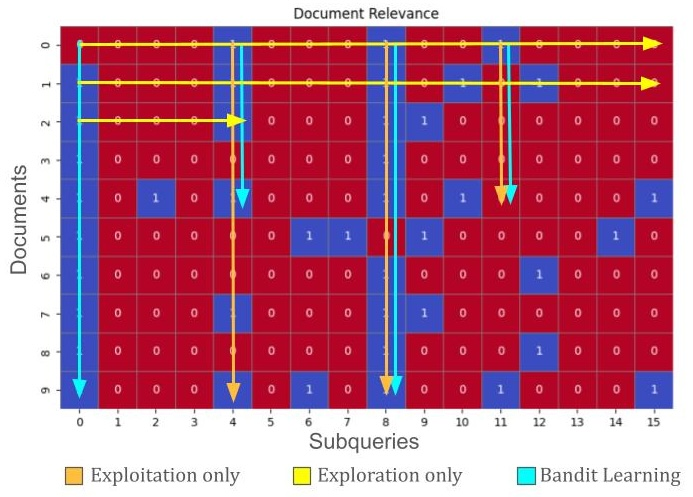
\includegraphics[width=\linewidth]{images/informative_subqueries_second_2.jpg}
    \caption{Exploration–exploitation across \(n\) subqueries and \(m\) documents; colors indicate document relevance, and arrows show how exploitation, exploration, and bandit-based policies allocate effort across sub-queries.}
    \label{fig:informative_subqueries}
\end{figure}

\subsection{Bandit learning for query decomposition}
Figure \ref{fig:informative_subqueries} illustrates the setting of our problem: given a user request \(\mathcal{Q}\) and its decomposition \(\{q_1, q_2, \ldots, q_K\}\), we retrieve a ranked list of \(N\) documents for each sub-query \(q_i\) as \(\{d_{i, 1}, d_{i, 2}, \ldots, d_{i, N}\}\). We observe one document at a time -we retrieve a document, assess its relevance with respect to \(\mathcal{Q}\), and store it as an evaluated document- while trying to maximize observed relevance while not going over a budget of \(b\) documents, where \(b < N\cdot K\). We model each sub-query \(q_i\) as an arm, where its associated set \(\mathcal{D}_i\) has an unknown distribution over relevance labels w.r.t.\ \(\mathcal{Q}\). We treat each arm as an unknown distribution over \(\mathcal{D}_i\) for which we maintain a posterior over its expected utility. We initialize the distribution with an uninformative (flat) prior and update the posterior after each observation over \(\mathcal{D}_i\). We employ Thompson sampling, a standard multi-armed bandits (MAB) algorithm, both in discrete (Algorithm \ref{tab:thompson_discrete_space}) and continuous space (Algorithm \ref{tab:thompson_continuous_space}). 


% \begin{algorithm}[!t]
% \footnotesize
% \caption{Thompson Sampling in Discrete Space}\label{tab:thompson_discrete_space}
% \small
% \SetKwInOut{Input}{Input}
% \SetKwInOut{Output}{Output}
% \Input{Sub-queries $\mathcal{S} = \{s_1, \dots, s_K\}$}
% \Input{Budget $b$}
% \BlankLine

% \For{$i = 1,\dots,K$}{Define Beta priors $\alpha_i \gets 1,\; \beta_i \gets 1$}

% Initialize observation set: $\mathcal{O} \gets \emptyset$

% \For{$t = 1,\dots,b$}{
%     \For{$i = 1,\dots,K$}{
%         Sample from posterior $\theta_i \sim \text{Beta}(\alpha_i,\beta_i)$
%     }
%     Select arm (sub-query): $a_t \gets \arg\max_{i} \theta_i$

%     Pick next document $d_{a_t, n} \in \mathcal{D}_{a_t}$ where
%     \hspace{1em} \(n = \min \{ j \in \{ 1,\ldots,N \} \mid (a_t, j) \notin \mathcal{O} \}\)
    
%     Observe the likelihood: $r(a_t, n)$

%     Update posterior: \\
%    \hspace{1em} $\alpha_{a_t} \gets \alpha_{a_t} + r(a_t, n)$ \\
%    \hspace{1em} $\beta_{a_t} \gets \beta_{a_t} + (1 - r(a_t, n))$

%     Save observation \(\mathcal{O} \gets \mathcal{O} \cup \{(a_t, n)\}\)
% }
% \end{algorithm}

\begin{algorithm}[!t]
\footnotesize
\caption{Thompson Sampling in Discrete Space}
\label{tab:thompson_discrete_space}

\SetKwInOut{Input}{Input}
\SetKwInOut{Output}{Output}
\Input{Sub-queries $\mathcal{S}=\{s_1,\dots,s_K\}$; Budget $b$}
\BlankLine

\For{$i=1,\dots,K$}{
  Define Beta priors $\alpha_i \gets 1,\; \beta_i \gets 1$
}

Initialize observation set $\mathcal{O} \gets \emptyset$\;

\For{$t=1,\dots,b$}{
  \For{$i=1,\dots,K$}{
    Sample $\theta_i \sim \mathrm{Beta}(\alpha_i,\beta_i)$
  }
  Select arm $a_t \gets \arg\max_i \theta_i$\;

  Pick next document $d_{a_t,n} \in \mathcal{D}_{a_t}$ where\\
  \hspace{1em}$n \gets \min\{\, j\in\{1,\ldots,N\}\mid (a_t,j)\notin\mathcal{O}\,\}$\;

  Observe reward $r(a_t,n)$\;

  Update posterior:\\
  \hspace{1em}$\alpha_{a_t} \gets \alpha_{a_t} + r(a_t,n)$; \quad
  $\beta_{a_t} \gets \beta_{a_t} + (1 - r(a_t,n))$\;

  Save observation $\mathcal{O} \gets \mathcal{O} \cup \{(a_t,n)\}$\;
}
\end{algorithm}


In discrete space, we model a Bernoulli distribution with a Beta conjugate prior, while in continuous space, we model Gaussians with Gaussian priors. Importantly, (i) we model the multi-armed bandit problem on query decomposition, where the arm chosen at time \(t\) is denoted as \(a_t\), (ii) each observation is represented by the next document \(d_{:,j}\) down a ranked list,
%for the chosen arm (sub-query)
and (iii) the reward is calculated at the document level, i.e., \(d_{{a_t}, j}\) for the chosen arm \(a_t\) and document rank \(j\). 

\subsection{Methods and rewards}\label{sec:rewards}
We study different properties that we hypothesize to play an important role in the task of sub-query-dependent document retrieval for RAG:

% \begin{enumerate}[leftmargin=*,nosep]
%     \item \textbf{Rank information}: Each sub-query \(q_i\) is associated with a ranked list of retrieved documents, whose order encodes an implicit estimate of relevance. To incorporate this rank-based signal, we calculate the reward for the sub-query chosen at time \(t\) as the average relevance over a local window of \(k\) documents down the ranked list: \(\frac{1}{k} \sum_{i=n}^{n+k-1} \text{Relevance}(d_{a_t, i})\), where \(d_{a_t, i}\) represents the \(i\)-th document retrieved for subquery chosen at action \(a_t\), \(n\) is the current position in the ranked list, and $\text{Relevance}(d_{a_t, i})$ represents the relevance of one document, either as a binary label (from human or LLM judges), or a continuous relevance signal (ranking score).
%     \item \textbf{Diversity of documents}: We want the retrieved documents to be diverse; retrieving a relevant document that has a high content overlap with a previously observed one does not bring new information. To encourage this, we estimate the novelty of the currently observed document \(d_{a_t, i}\) with respect to the set of previously observed documents \(\mathcal{O}\); we model this by estimating the novelty of each sub-query using cosine similarity: \(1 - \frac{\max_{(i, j) \in \mathcal{O}} \cos(d_{a_t, n}, d_{i, j}) + 1}{2}\).
%     \item \textbf{Exploration}: We want each sub-query to be explored; we enforce this using an upper confidence bound (UCB) term \(c \cdot \sqrt{\frac{1}{n}\log_2(n + 1)}\), with \( c \to 0 \). This term diverges to infinity for subqueries for which no observations have been done, i.e., when \(n\rightarrow0\).
% \end{enumerate}

\noindent\textbf{Rank information}: Each sub-query \(q_i\) is associated with a ranked list of retrieved documents, whose order encodes an implicit estimate of relevance. To incorporate this rank-based signal, we calculate the reward for the sub-query \(a_t\) chosen at time \(t\) as the average relevance over a local window of \(k\) documents down the ranked list: \(\frac{1}{k} \sum_{i=n}^{n+k-1} \text{Relevance}(d_{a_t, i})\), where \(d_{a_t, i}\) represents the \(i\)-th document retrieved for subquery chosen at time \(t\), \(n\) is the current position in the ranked list, and $\text{Relevance}(d_{a_t, i})$ represents the relevance of one document, either as a binary label (from human or LLM judges), or a continuous relevance signal (ranking score).

\noindent\textbf{Diversity of documents}: We want the retrieved documents to be diverse; retrieving a relevant document that has a high content overlap with a previously observed one does not bring new information. To encourage this, we estimate the novelty of the currently observed document \(d_{a_t, i}\) with respect to the set of previously observed documents \(\mathcal{O}\); we model this by estimating the novelty of each sub-query using cosine similarity: \(1 - \frac{\max_{(i, j) \in \mathcal{O}} \cos(d_{a_t, n}, d_{i, j}) + 1}{2}\).

\noindent\textbf{Exploration}: We want to explore each sub-at least once; we enforce this using an upper confidence bound (UCB) term \(c \cdot \sqrt{\frac{1}{n}\log_2(n + 1)}\), with \( c \to 0 \). This term diverges to infinity for subqueries with no observations, i.e., when \(n\rightarrow0\).


\noindent%
These factors compose our final reward policy, which we propose as a Bernoulli top-$k$ UCB diversity-aware estimate in Eq.~\ref{eq:top_reward}, used on line 9 in Algorithm \ref{tab:thompson_discrete_space}: 
%
\begin{equation}
\begin{split}
r(a_t, & \,n) = {}\\
& \frac{1}{k} \sum_{i=n}^{n+k-1} \text{Relevance}(d_{a_t, i}) \cdot {} \\
& \left( 1 -
    \frac{\max\limits_{(i, j) \in \mathcal{O}} \cos(d_{a_t, n}, d_{i, j}) + 1}{2} \right) \\
& {}+ c \cdot \sqrt{\frac{\log_2(n + 1)}{n}}, 
 \text{ with } c \to 0.
\end{split} 
\label{eq:top_reward}
\end{equation}
% We consider multiple variants and baselines as described in Table \ref{tab:reward_functions}. 

% \begin{table*}[!t]
% \centering
% \setlength{\tabcolsep}{1.5pt}
% \resizebox{\textwidth}{!}{%
% \begin{tabular}{ll}
%     \toprule
%     \textbf{Reward type} & \textbf{Formula} \\
    
%     \midrule

%     Baseline random & \(r(a_t) = \text{Relevance}(d_{a_t, n})\) \text{ where} \(a_t \sim \text{unif}(a_1, ..., a_K), n \sim \text{unif}(rank_1, rank_2, .. rank_m)\) \\[0.5em]
    
%     Baseline random rank-aware & \(r(a_t, n) = \text{Relevance}(d_{a_t}, n)\) \text{ where} \(a_t \sim \text{unif}(a_1, ..., a_K)\) \\[0.5em]

%     \midrule
%     \(\epsilon\)-greedy & \(r(a_t, n) = \text{Relevance}(d_{a_t, n})\) \text{ if} \(\text{Relevance}(d_{a_t, n-1})\) \text{ is 1 else } \(a_t \sim \text{unif}(a_1, ..., a_K)\) \\[0.5em]
    
%     Bernoulli & \( r(a_t, n) = \text{Relevance}(d_{a_t, n}) \) \\[0.5em]
    
%     Bernoulli UCB & \( r(a_t, n) = \text{Relevance}(d_{a_t, n}) + c \cdot \sqrt{\frac{\log_2(n + 1)}{n}} \quad \text{with } c \to 0 \) \\[0.5em]
    
%     Bernoulli top-\(k\) & \( r(a_t, n) = \frac{1}{k} \sum_{i=n}^{n+k-1} \text{Relevance}(d_{a_t, i}) \) \\[0.5em]
    
%     Bernoulli rank-aware & \( r(a_t, n) = \frac{\text{Relevance}(d_{a_t, n})}{\log_2(n + 2)} \) \\[0.5em]
    
%     Gaussian & \( r(a_t, n) = \text{RFF}(d_{a_t, n}) \quad \text{or} \quad \text{ColBERT}(d_{a_t, n}) \) \\[0.5em]
    
%     Diversity & \( r(a_t, n) = \text{Relevance}(d_{a_t, n}) \cdot \left(1 - \frac{\max\limits_{(i, j) \in \mathcal{O}} \cos(d_{a_t, n}, d_{i, j}) + 1}{2}\right) \) \\[0.5em]
    
%     Diversity concave & \(
%     r(a_t, n) = \text{Relevance}(d_{a_t, n}) \cdot 
%     \begin{cases}
%     1, & \text{if } \max\limits_{j < n} \cos(d_{a_t, n}, d_{a_t, j}) < 0 \\
%     \exp\left(-a \cdot \left(\max\limits_{(i, j) \in \mathcal{O}} \cos(d_{a_t, n}, d_{i, j}))\right)^b\right), & \text{otherwise}
%     \end{cases}
%     \)  \\[0.5em]

%     Bernoulli top-\(k\) UCB diversity & \( r(a_t, n) = \frac{1}{k} \sum_{i=n}^{n+k-1} \text{Relevance}(d_{a_t, i}) \cdot \left(1 - \frac{\max\limits_{(i, j) \in \mathcal{O}} \cos(d_{a_t, n}, d_{i, j})) + 1}{2}\right) + c \cdot \sqrt{\frac{\log_2(n + 1)}{n}}, \text{ with } c \to 0 \)\\
%     \bottomrule
%     \end{tabular} }
%     \caption{Reward functions used for evaluating sub-query selection strategies. For all but the baseline random, we assume \(n = \min \{ j \in \{1,\ldots,N\} \mid (a_t, j) \notin \mathcal{O} \}\). For Diversity Concave policy, we assume \(a=5\) and \(b=15\).}
% \label{tab:reward_functions}
% \end{table*}

\subsection{Hierarchical query decomposition with Correlated MAB}\label{sec:hierarchical_method}

%% What are correlated bandits
In hierarchical decompositions, a complex user request is iteratively split into smaller subqueries, where each can be further decomposed into more fine-grained information needs (see Figure \ref{fig:query_decomposition_herarchical}). As a result, the retrieval space forms a hierarchy of sub-queries and their associated document distributions, where each child sub-query inherits properties from its parent. As some sub-queries may be more informative than others, instead of uniform expansion, we selectively expand those that demonstrate high utility according to their posterior estimates. A sub-query \(q_i\) is highly informative when its estimated value is above a set informativeness threshold \(\mathbb{E}_{q_i} = \frac{\alpha_i}{\alpha_i + \beta_i} > \tau\) and when it has been observed at least \(n\) times. If an informative sub-query \(q_i\) is expanded, its children \(\{q_{i, 1}, q_{i, 2}, ..., q_{i, m}\}\) become new arms in the multi-armed bandit formalization, whose distributions are correlated with their parent sub-query \(q_i\). This correlation is captured by an inheritance factor \(\lambda \in (0, 1]\), i.e. a parent with posterior \(\text{Beta}(\alpha_i, \beta_i)\) will yield a child sub-query initialized as \(\text{Beta}(\lambda \alpha_i, \lambda \beta_i)\). 

% In a setting where the user request is first decomposed into sub-queries, and each sub-query can be further decomposed into second-level sub-queries, we obtain a \textbf{hierarchical decomposition} of a complex user request into unitary information needs (see Figure \ref{fig:query_decomposition_herarchical}). In this case, the document distribution associated with each second-level sub-query is dependent on its parent sub-query. Assuming an initial decomposition setting, %where we first decompose the user request into one level of sub-queries, while observing documents and building estimated over the utility of each, 
% one might observe that some sub-queries are more informative than others. In such cases, it may be preferable to further decompose the informative sub-queries rather than explore entirely new ones. The resulting decomposition creates new arms in the multi-armed bandit, with distributions that are unknown but correlated with their parent. This correlation can be modeled by transmitting information learned from the parent to its children. We update Algorithms \ref{tab:thompson_discrete_space} and \ref{tab:thompson_continuous_space} to model correlated bandits as follows:

% \begin{enumerate}[leftmargin=*,nosep]
%     \item Check how many times each arm has been observed. If a sub-query \(q_i\) has been observed more than a fixed threshold \(n\), and if it is informative enough, i.e., \(\mathbb{E}_{q_i} = \frac{\alpha_i}{\alpha_i + \beta_i} > \tau\), we decompose the query.
%     \item We add the new sub-queries as arms and initialized them as \(\alpha_{i,j} \gets \lambda \cdot \alpha_i\), \(\beta_{i,j} \gets \lambda \cdot \beta_i\).
% \end{enumerate}


%% In our setup: figure
\begin{figure}[!t]
    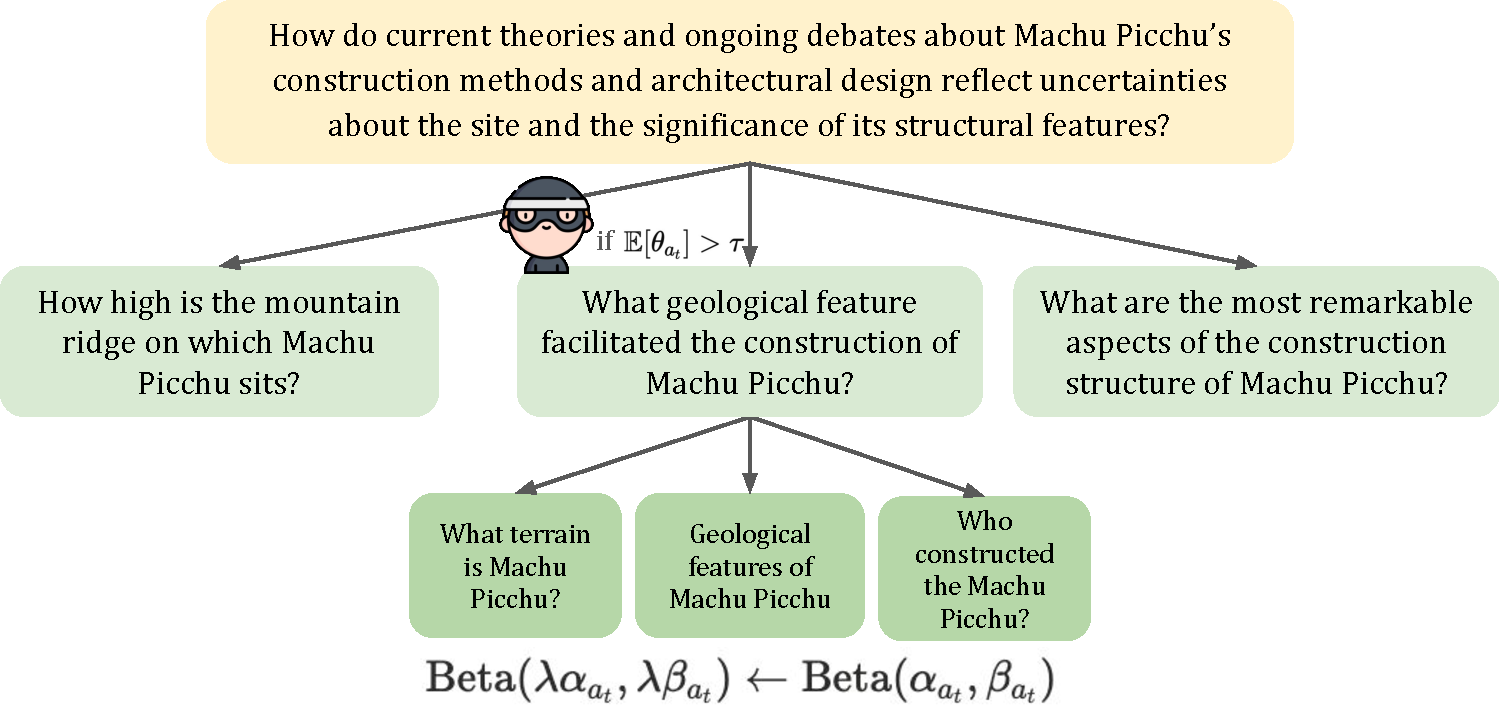
\includegraphics[width=\linewidth]{images/correlated_bandits_2.pdf}
    \caption{Hierarchical query decomposition with correlated bandits, where informative sub-queries are decomposed into arms with inherited posterior beliefs.}
    \label{fig:query_decomposition_herarchical}
\end{figure}
